% move all configuration stuff into includes file so we can focus on the content
\documentclass[aspectratio=169,hyperref={pdfpagelabels=false,colorlinks=true,linkcolor=white,urlcolor=blue},t]{beamer}

%%%%%%%%%%%%%%%%%%%%%%%%%%%%%%%%%%%%%%%%%%%%%%%%%%%%%%%%%%%%%%%%%%%%%%%%%%%%%%%%%%
%%%%%%%%%%%%%%%%%%%%%%%%%%%%%%%%%%%%%%%%%%%%%%%%%%%%%%%%%%%%%%%%%%%%%%%%%%%%%%%%%%
% packages
\usepackage{pict2e}
\usepackage{epic}
\usepackage{amsmath,amsfonts,amssymb}
\usepackage{units}
\usepackage{fancybox}
\usepackage[absolute,overlay]{textpos} 
\usepackage{media9} % avi2flv: "C:\Program Files\ffmpeg\bin\ffmpeg.exe" -i TuneFreqFilterbank.avi -b 600k -s 441x324 -r 15 -acodec copy TuneFreqFilterbank.flv
\usepackage{animate}
\usepackage{gensymb}
\usepackage{multirow}
\usepackage{silence}
\usepackage{tikz}
\usepackage[backend=bibtex,style=ieee]{biblatex}
\AtEveryCitekey{\iffootnote{\tiny}{}}
\addbibresource{include/references}

%%%%%%%%%%%%%%%%%%%%%%%%%%%%%%%%%%%%%%%%%%%%%%%%%%%%%%%%%%%%%%%%%%%%%%%%%%%%%%%%%%
%%%%%%%%%%%%%%%%%%%%%%%%%%%%%%%%%%%%%%%%%%%%%%%%%%%%%%%%%%%%%%%%%%%%%%%%%%%%%%%%%%
% relative paths
\graphicspath{{graph/}}


%%%%%%%%%%%%%%%%%%%%%%%%%%%%%%%%%%%%%%%%%%%%%%%%%%%%%%%%%%%%%%%%%%%%%%%%%%%%%%%%%%
%%%%%%%%%%%%%%%%%%%%%%%%%%%%%%%%%%%%%%%%%%%%%%%%%%%%%%%%%%%%%%%%%%%%%%%%%%%%%%%%%%
% units
\setlength{\unitlength}{1mm}

%%%%%%%%%%%%%%%%%%%%%%%%%%%%%%%%%%%%%%%%%%%%%%%%%%%%%%%%%%%%%%%%%%%%%%%%%%%%%%%%%%
%%%%%%%%%%%%%%%%%%%%%%%%%%%%%%%%%%%%%%%%%%%%%%%%%%%%%%%%%%%%%%%%%%%%%%%%%%%%%%%%%%
% theme & layout
\usetheme{Frankfurt}
\beamertemplatenavigationsymbolsempty
%\setbeamertemplate{frametitle}[smoothbars theme]
\setbeamertemplate{frametitle}
{
    \begin{beamercolorbox}[ht=1.8em,wd=\paperwidth]{frametitle}
        \vspace{-.1em}%
        \hspace{.2em}{\strut\insertframetitle\strut}
        
        \hspace{.2em}\small\strut\insertframesubtitle\strut
        %\hfill
        %\includegraphics[height=.8cm,keepaspectratio]{CenterMusicTechnology-solid-2lines-white-CoAtag}
        
    \end{beamercolorbox}
    \begin{textblock*}{100mm}(11.6cm,.7cm)
        \includegraphics[height=.8cm,keepaspectratio]{Logo_GTCMT_black}
    \end{textblock*}
}
\setbeamertemplate{footline}[frame number]

% set this to ensure bulletpoints without subsections
\usepackage{remreset}
\makeatletter
\@removefromreset{subsection}{section}
\makeatother
\setcounter{subsection}{1}

%---------------------------------------------------------------------------------
% appearance
\setbeamercolor{structure}{fg=gtgold}
\setbeamercovered{transparent} %invisible
\setbeamercolor{bibliography entry author}{fg=black}
\setbeamercolor*{bibliography entry title}{fg=black}
\setbeamercolor*{bibliography entry note}{fg=black}
\setbeamercolor{frametitle}{fg=black}
\setbeamercolor{title}{fg=black}

%\usepackage{pgfpages}
%\setbeameroption{show notes}
%\setbeameroption{show notes on second screen=right}
%---------------------------------------------------------------------------------
% fontsize
\let\Tiny=\tiny

%%%%%%%%%%%%%%%%%%%%%%%%%%%%%%%%%%%%%%%%%%%%%%%%%%%%%%%%%%%%%%%%%%%%%%%%%%%%%%%%%%
%%%%%%%%%%%%%%%%%%%%%%%%%%%%%%%%%%%%%%%%%%%%%%%%%%%%%%%%%%%%%%%%%%%%%%%%%%%%%%%%%%
% warnings
\pdfsuppresswarningpagegroup=1
\WarningFilter{biblatex}{Patching footnotes failed}
\WarningFilter{latexfont}{Font shape}
\WarningFilter{latexfont}{Some font shapes}
\WarningFilter{gensymb}{Not defining}


%%%%%%%%%%%%%%%%%%%%%%%%%%%%%%%%%%%%%%%%%%%%%%%%%%%%%%%%%%%%%%%%%%%%%%%%%%%%%%%%%%
%%%%%%%%%%%%%%%%%%%%%%%%%%%%%%%%%%%%%%%%%%%%%%%%%%%%%%%%%%%%%%%%%%%%%%%%%%%%%%%%%%
% theme & layout
\usetheme{Frankfurt}
\useinnertheme{rectangles}


%%%%%%%%%%%%%%%%%%%%%%%%%%%%%%%%%%%%%%%%%%%%%%%%%%%%%%%%%%%%%%%%%%%%%%%%%%%%%%%%%%
\setbeamertemplate{frametitle}[default][colsep=-4bp,rounded=false,shadow=false]
\setbeamertemplate{frametitle}
{%
    \nointerlineskip%
    %\vskip-0.5ex
    \begin{beamercolorbox}[wd=\paperwidth,ht=3.5ex,dp=0.6ex]{frametitle}
        \hspace*{1.3ex}\insertframetitle%
        
        \hspace*{1.3ex}\small\insertframesubtitle%
    \end{beamercolorbox}%
    \begin{textblock*}{100mm}(11.6cm,.57cm)
        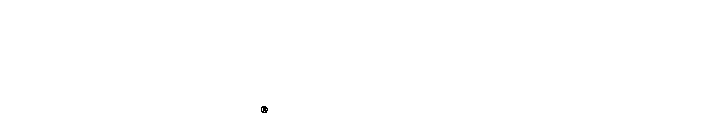
\includegraphics[height=.8cm,keepaspectratio]{graph/Logo_GTCMT_white}
    \end{textblock*}
}


%%%%%%%%%%%%%%%%%%%%%%%%%%%%%%%%%%%%%%%%%%%%%%%%%%%%%%%%%%%%%%%%%%%%%%%%%%%%%%%%%%
\setbeamertemplate{title page}[default][colsep=-4bp,rounded=false,shadow=false]
\setbeamertemplate{title page}
{
    \begin{textblock*}{100mm}(15cm,.51cm)
            \href{https://github.com/alexanderlerch/ACA-Slides/blob/2nd_edition/\jobname.pdf}{\includegraphics[height=.5cm,keepaspectratio]{graph/Logo_github}}\hspace*{2ex}
    \end{textblock*}
    \vskip-10ex
    \begin{beamercolorbox}[wd=\paperwidth,ht=.7\paperheight,dp=0.6ex]{frametitle} %35ex
        %\begin{flushright}
            %\href{http://www.gtcmt.gatech.edu}{\includegraphics[height=.8cm,keepaspectratio]{graph/Logo_GTCMT_black}}\hspace*{2ex}
        %\end{flushright}
        
        \hspace*{1.8ex}\LARGE\inserttitle%
        
        \vspace*{.5ex}
        
        \hspace*{1.3ex}\small\insertsubtitle%
        
        \vspace*{.5ex}
    \end{beamercolorbox}%
    \nointerlineskip%
    \begin{beamercolorbox}[wd=\paperwidth,ht=.4\paperheight,dp=0.6ex]{page number in head/foot}
        %\vspace*{-.5ex}
        \hspace*{1.7ex}\small\insertauthor%
        
        %\hspace*{1.7ex}\small }%
        
        \vspace*{10ex}
        
        \begin{flushright}
            \href{http://www.gtcmt.gatech.edu}{\includegraphics[height=.8cm,keepaspectratio]{graph/Logo_GTCMT_black}}\hspace*{2ex}
        \end{flushright}
    \end{beamercolorbox}%
}


%%%%%%%%%%%%%%%%%%%%%%%%%%%%%%%%%%%%%%%%%%%%%%%%%%%%%%%%%%%%%%%%%%%%%%%%%%%%%%%%%%
%\makeatother
\setbeamertemplate{footline}
{
  \leavevmode%
  \hbox{%
  \begin{beamercolorbox}[wd=.5\paperwidth,ht=2.25ex,dp=1ex,left,leftskip=1ex]{page number in head/foot}%
    \insertsubtitle
  \end{beamercolorbox}%
  \begin{beamercolorbox}[wd=.5\paperwidth,ht=2.25ex,dp=1ex,right,rightskip=1ex]{page number in head/foot}%
    \hfill
    \insertframenumber{} / \inserttotalframenumber
  \end{beamercolorbox}}%
  \vskip0pt%
}
%\makeatletter


%%%%%%%%%%%%%%%%%%%%%%%%%%%%%%%%%%%%%%%%%%%%%%%%%%%%%%%%%%%%%%%%%%%%%%%%%%%%%%%%%%
\beamertemplatenavigationsymbolsempty
\setbeamertemplate{navigation symbols}{}
\setbeamertemplate{blocks}[default]%[rounded=false,shadow=false]
\setbeamertemplate{itemize item}[square]
\setbeamertemplate{itemize subitem}[circle]
\setbeamertemplate{itemize subsubitem}[triangle]
\setbeamertemplate{enumerate item}[square]
\setbeamertemplate{enumerate subitem}[circle]
\setbeamertemplate{enumerate subsubitem}[circle]


%%%%%%%%%%%%%%%%%%%%%%%%%%%%%%%%%%%%%%%%%%%%%%%%%%%%%%%%%%%%%%%%%%%%%%%%%%%%%%%%%%
% colors
\setbeamercolor{structure}{fg=darkgray}
\setbeamercovered{transparent} %invisible
\setbeamercolor{bibliography entry author}{fg=black}
\setbeamercolor*{bibliography entry title}{fg=black}
\setbeamercolor*{bibliography entry note}{fg=black}
\setbeamercolor{frametitle}{fg=black}
\setbeamercolor{title}{fg=white}
\setbeamercolor{subtitle}{fg=white}
\setbeamercolor{frametitle}{fg=white}
\setbeamercolor{framesubtitle}{fg=white}
\setbeamercolor{mini frame}{fg=white, bg=black}
\setbeamercolor{section in head/foot}{fg=white, bg=darkgray}
\setbeamercolor{page number in head/foot}{fg=black, bg=lightblue}
\setbeamercolor{item projected}{fg=white, bg=black}

%---------------------------------------------------------------------------------
%%%%%%%%%%%%%%%%%%%%%%%%%%%%%%%%%%%%%%%%%%%%%%%%%%%%%%%%%%%%%%%%%%%%%%%%%%%%%%%%%%
%%%%%%%%%%%%%%%%%%%%%%%%%%%%%%%%%%%%%%%%%%%%%%%%%%%%%%%%%%%%%%%%%%%%%%%%%%%%%%%%%%
% title information
\title[]{Introduction to \textbf{Audio Content Analysis}}   
\author[alexander lerch]{alexander lerch} 
%\institute{~}
%\date[Alexander Lerch]{}
%\titlegraphic{\vspace{-16mm}\includegraphics[width=\textwidth,height=3cm]{title}}

%%%%%%%%%%%%%%%%%%%%%%%%%%%%%%%%%%%%%%%%%%%%%%%%%%%%%%%%%%%%%%%%%%%%%%%%%%%%%%%%%%
%%%%%%%%%%%%%%%%%%%%%%%%%%%%%%%%%%%%%%%%%%%%%%%%%%%%%%%%%%%%%%%%%%%%%%%%%%%%%%%%%%
% colors
\definecolor{gtgold}{HTML}{E0AA0F} %{rgb}{0.88,0.66,1,0.06} [234, 170, 0]/256
\definecolor{darkgray}{rgb}{.1, .1, .25}
\definecolor{lightblue}{rgb}{.1, 0.75, 1}
\definecolor{highlight}{rgb}{0, 0, 1} %_less!40

%%%%%%%%%%%%%%%%%%%%%%%%%%%%%%%%%%%%%%%%%%%%%%%%%%%%%%%%%%%%%%%%%%%%%%%%%%%%%%%%%%
%%%%%%%%%%%%%%%%%%%%%%%%%%%%%%%%%%%%%%%%%%%%%%%%%%%%%%%%%%%%%%%%%%%%%%%%%%%%%%%%%%
% relative paths
\graphicspath{{../ACA-Plots/graph/}}


%%%%%%%%%%%%%%%%%%%%%%%%%%%%%%%%%%%%%%%%%%%%%%%%%%%%%%%%%%%%%%%%%%%%%%%%%%%%%%%%%%
%%%%%%%%%%%%%%%%%%%%%%%%%%%%%%%%%%%%%%%%%%%%%%%%%%%%%%%%%%%%%%%%%%%%%%%%%%%%%%%%%%
% units
\setlength{\unitlength}{1mm}

%%%%%%%%%%%%%%%%%%%%%%%%%%%%%%%%%%%%%%%%%%%%%%%%%%%%%%%%%%%%%%%%%%%%%%%%%%%%%%%%%%
%%%%%%%%%%%%%%%%%%%%%%%%%%%%%%%%%%%%%%%%%%%%%%%%%%%%%%%%%%%%%%%%%%%%%%%%%%%%%%%%%%
% math
\DeclareMathOperator*{\argmax}{argmax}
\DeclareMathOperator*{\argmin}{argmin}
\DeclareMathOperator*{\atan}{atan}
\DeclareMathOperator*{\arcsinh}{arcsinh}
\DeclareMathOperator*{\sign}{sign}
\DeclareMathOperator*{\tcdf}{tcdf}
\DeclareMathOperator*{\si}{sinc}
\DeclareMathOperator*{\princarg}{princarg}
\DeclareMathOperator*{\arccosh}{arccosh}
\DeclareMathOperator*{\hwr}{HWR}
\DeclareMathOperator*{\flip}{flip}
\DeclareMathOperator*{\sinc}{sinc}
\DeclareMathOperator*{\floor}{floor}
\newcommand{\e}{{e}}
\newcommand{\jom}{\mathrm{j}\omega}
\newcommand{\jOm}{\mathrm{j}\Omega}
\newcommand   {\mat}[1]    		{\boldsymbol{\uppercase{#1}}}		%bold
\renewcommand {\vec}[1]    		{\boldsymbol{\lowercase{#1}}}		%bold

%%%%%%%%%%%%%%%%%%%%%%%%%%%%%%%%%%%%%%%%%%%%%%%%%%%%%%%%%%%%%%%%%%%%%%%%%%%%%%%%%%
%%%%%%%%%%%%%%%%%%%%%%%%%%%%%%%%%%%%%%%%%%%%%%%%%%%%%%%%%%%%%%%%%%%%%%%%%%%%%%%%%%
% media9
\newcommand{\includeaudio}[1]{
\href{run:audio/#1.mp3}{
\includegraphics[width=5mm, height=5mm]{graph/SpeakerIcon}}}

\newcommand{\includeanimation}[4]{{\begin{center}
                        \animategraphics[autoplay,loop,scale=.7]{#4}{animation/#1-}{#2}{#3}        
                        \end{center}
                        \addreference{matlab source: \href{https://github.com/alexanderlerch/ACA-Plots/blob/master/matlab/animate#1.m}{matlab/animate#1.m}}}
                        \inserticon{video}}
                        
%%%%%%%%%%%%%%%%%%%%%%%%%%%%%%%%%%%%%%%%%%%%%%%%%%%%%%%%%%%%%%%%%%%%%%%%%%%%%%%%%%
%%%%%%%%%%%%%%%%%%%%%%%%%%%%%%%%%%%%%%%%%%%%%%%%%%%%%%%%%%%%%%%%%%%%%%%%%%%%%%%%%%
% other commands
\newcommand{\question}[1]{%\vspace{-4mm}
                          \setbeamercovered{invisible}
                          \begin{columns}[T]
                            \column{.9\textwidth}
                                \textbf{#1}
                            \column{.1\textwidth}
                                \vspace{-8mm}
                                \begin{flushright}
                                     
\includegraphics[width=.9\columnwidth]{graph/question_mark}
                                \end{flushright}
                                \vspace{6mm}
                          \end{columns}\pause\vspace{-12mm}}

\newcommand{\toremember}[1]{
                        \inserticon{lightbulb}
                        }

\newcommand{\matlabexercise}[1]{%\vspace{-4mm}
                          \setbeamercovered{invisible}
                          \begin{columns}[T]
                            \column{.8\textwidth}
                                \textbf{matlab exercise}: #1
                            \column{.2\textwidth}
                                \begin{flushright}
                                     \includegraphics[scale=.5]{graph/logo_matlab}
                                \end{flushright}
                                %\vspace{6mm}
                          \end{columns}}

\newcommand{\addreference}[1]{  
                  
                    \begin{textblock*}{\baselineskip }(.98\paperwidth,.5\textheight) %(1.15\textwidth,.4\textheight)
                         \begin{minipage}[b][.5\paperheight][b]{1cm}%
                            \vfill%
                             \rotatebox{90}{\tiny {#1}}
                        \end{minipage}
                   \end{textblock*}
                    }
                    
\newcommand{\figwithmatlab}[1]{
                    \begin{figure}
                        \centering
                        \includegraphics[scale=.7]{#1}
                        %\label{fig:#1}
                    \end{figure}
                    
                    \addreference{matlab source: \href{https://github.com/alexanderlerch/ACA-Plots/blob/main/matlab/plot#1.m}{plot#1.m}}}
\newcommand{\figwithref}[2]{
                    \begin{figure}
                        \centering
                        \includegraphics[scale=.7]{#1}
                        \label{fig:#1}
                    \end{figure}
                    
                    \addreference{#2}}  
                                    
\newcommand{\inserticon}[1]{
                    \begin{textblock*}{100mm}(14.5cm,7.5cm)
                        \includegraphics[height=.8cm,keepaspectratio]{graph/#1}
                    \end{textblock*}}            

%%%%%%%%%%%%%%%%%%%%%%%%%%%%%%%%%%%%%%%%%%%%%%%%%%%%%%%%%%%%%%%%%%%%%%%%%%%%%%%%%%
%%%%%%%%%%%%%%%%%%%%%%%%%%%%%%%%%%%%%%%%%%%%%%%%%%%%%%%%%%%%%%%%%%%%%%%%%%%%%%%%%%
% counters
\newcounter{i}
\newcounter{j}
\newcounter{iXOffset}
\newcounter{iYOffset}
\newcounter{iXBlockSize}
\newcounter{iYBlockSize}
\newcounter{iYBlockSizeDiv2}
\newcounter{iXBlockSizeDiv2}
\newcounter{iDistance}




\subtitle{Module A.3: Fundamentals~---~Correlation}

%%%%%%%%%%%%%%%%%%%%%%%%%%%%%%%%%%%%%%%%%%%%%%%%%%%%%%%%%%%%%%%%%%%%%%%%%%%%
\begin{document}
    % generate title page
	{
\setbeamertemplate{headline}{} 
\setbeamertemplate{footline}{} 
\begin{frame}
    \titlepage
    %\vspace{-5mm}
\end{frame}
}
\addtocounter{framenumber}{-1}


    \section[overview]{lecture overview}
        \begin{frame}{introduction}{overview}
            \begin{block}{corresponding textbook section}
                    %\href{http://ieeexplore.ieee.org/xpl/articleDetails.jsp?tp=&arnumber=6331119&}{Chapter 2~---~Fundamentals}: pp.~24--28
                    Appendix A.3
            \end{block}

            \begin{itemize}
                \item   \textbf{lecture content}
                    \begin{itemize}
                        \item   cross correlation function (CCF)
                        \item   auto-correlation function (ACF)
                    \end{itemize}
                \bigskip
                \item<2->   \textbf{learning objectives}
                    \begin{itemize}
                        \item   describe use cases of correlation
                        \item   implement cross- and auto-correlation
                    \end{itemize}
            \end{itemize}
            \inserticon{directions}
        \end{frame}

    \section[CCF]{cross correlation function}
        \begin{frame}{correlation function}{definition}
            \textbf{correlation function}: compute similarity between two \textit{stationary} signals $x$,$y$
            \begin{equation*}
                r_\mathrm{xy}(\tau)=\mathcal{E}\lbrace x(t)y(t+\tau)\rbrace  
            \end{equation*}  
            
            \begin{itemize}
                \item	\textbf{continuous}:
                    \begin{equation*}
                        r_\mathrm{xy}(\tau) = \int\limits_{-\infty}^{\infty}{x(t)\cdot y(t+\tau)dt}
                    \end{equation*}
                \item	\textbf{discrete}:
                    \begin{equation*}
                        r_\mathrm{xy}(\eta) = \sum\limits_{i=-\infty}^{\infty}{x(i)\cdot y(i+\eta)}
                    \end{equation*}
            \end{itemize}
        \end{frame}	

        \begin{frame}{correlation function}{animation}
            \vspace{-5mm}
            \begin{footnotesize}
                    \begin{equation*}
                        %r_\mathrm{xy}(\tau) &=& \int\limits_{-\infty}^{\infty}{x(t)\cdot y(t+\tau)dt}\\
                        r_\mathrm{xy}(\eta) = \sum\limits_{i=-\infty}^{\infty}{x(i)\cdot y(i+\eta)}
                    \end{equation*}
            \end{footnotesize}
            \includeanimation
                {Correlation}
                {000}
                {250}
                {10}
            %\begin{center}
                %\animategraphics[loop]{10}{animateCorrelation/Correlation-}{000}{250}        
            %\end{center}
            %\addreference{matlab source: \href{https://github.com/alexanderlerch/ACA-Slides/blob/master/matlab/animateCorrelation.m}{matlab/animateCorrelation.m}}
            \inserticon{video}
        \end{frame}

    \section[blocked correlation]{blocked cross correlation function}
        \begin{frame}{correlation function}{examples}
			\begin{itemize}
				\item	rectangular window vs.
				\item	sine vs.
				\item	noise
			\end{itemize}
            \vspace{-5mm}
            \figwithmatlab{Correlation}
        \end{frame}	

        \begin{frame}{correlation function}{blocked correlation: animation}
            \includeanimation
                {BlockedCorrelation}
                {001}
                {1023}
                {24}
            %\begin{center}
                %\animategraphics[loop]{24}{animateBlockedCorrelation/BlockedCorrelation-}{001}{1023}        
            %\end{center}
            %\addreference{matlab source: \href{https://github.com/alexanderlerch/ACA-Slides/blob/master/matlab/animateBlockedCorrelation.m}{matlab/animateBlockedCorrelation.m}}
            \inserticon{video}
        \end{frame}	 

    \section[normalization]{normalization of blocked correlation}
        \begin{frame}{correlation function}{normalization}
        \vspace{-3mm}
            \begin{equation*}\label{eq:corrnorm}
                \lambda_c = \frac{1}{\sqrt{\left(\sum\limits_{i=i_{\mathrm{s}}(n)}^{i_{\mathrm{e}}(n)}{x^2(i)}\right)\cdot \left(\sum\limits_{i=i_{\mathrm{s}}(n)}^{i_{\mathrm{e}}(n)}{y^2(i)}\right)}} 
            \end{equation*}
            
            \bigskip
            methods of dealing with the triangular weighting/shape for blocked correlation:
            \begin{enumerate}
                \item<2->	different block lengths ($\mathcal{K},3\mathcal{K})$
                \item<2->	circular application
                \item<2->	modified normalization
                    \begin{equation*}
                        \lambda_c(\eta) = \frac{\mathcal{K}}{(\mathcal{K}-|\eta|)\cdot\sqrt{\left(\sum\limits_{i=i_{\mathrm{s}}(n)}^{i_{\mathrm{e}}(n)}{x^2(i)}\right)\cdot \left(\sum\limits_{i=i_{\mathrm{s}}(n)}^{i_{\mathrm{e}}(n)}{y^2(i)}\right)}} .
                    \end{equation*}
            \end{enumerate}
        \end{frame}	

    \section[ACF]{autocorrelation function}
        \begin{frame}{autocorrelation function}{definition \& properties}
            \toremember{}
            \begin{block}{autocorrelation function properties}
                \begin{itemize}
                    \item   ACF is correlation function with the signal itself $r_{xx}(\eta)$
                    \item	{ACF} at lag $0$:\\
                    $r_{xx}(0,n) = 1$ if normalized, energy otherwise
                
                    \item	maximum:\\
                    $|r_{xx}(\eta,n)| \leq r_{xx}(0,n)$ 
                    \item	symmetry:\\
                    $r_{xx}(\eta,n) = r_{xx}(-\eta,n)$
                    \item	periodicity:\\
                    The {ACF} of a periodic signal is periodic (period length of input signal)
                \end{itemize}	
            \end{block}
        \end{frame}	

    \section[apps]{applications}
        \begin{frame}{(auto-)correlation function}{applications and use cases}
            \question{what are the use cases of correlation}
            
            \begin{itemize}
                \item   \textit{cross-correlation}:
                    \begin{itemize}
                        \item   compute similarity between different signals (correlation meter)
                        \item   detect shift between two similar but shifted signals (radar)
                    \end{itemize}
                \bigskip
                \item   \textit{autocorrelation}:
                    \begin{itemize}
                        \item   detect self-similarity of (shifted) signal (lpc coefficients, noisiness)
                        \item   detect periodicity of signal
                    \end{itemize}
            \end{itemize}
        \end{frame}	
        
    \section{summary}
        \begin{frame}{summary}{lecture content}
            \begin{itemize}
                \item   \textbf{correlation function}
                    \begin{itemize}
                        \item   measure of similarity between two signals
                        \item   use case example: find time lag between signals
                    \end{itemize}
                \bigskip
                \item   \textbf{normalized correlation}
                    \begin{itemize}
                        \item   results in value between $-1\ldots 1$
                        \item   correlation coefficient: normalized correlation at lag $\eta=0$
                    \end{itemize}
                \bigskip
                \item   \textbf{autocorrelation}
                    \begin{itemize}
                        \item   measure of self-similarity
                        \item   use case example: find periodicity
                    \end{itemize}
            \end{itemize}
            \inserticon{summary}
        \end{frame}
\end{document}
